\section{Introduction}
% Machine learning workloads imply novel topologies
Recent trends in machine learning towards training and serving large models together with the stagnation of Moore's-law-induced compute performance has led system designers to include novel high-bandwidth interconnect networks both within and across nodes in distributed clusters. For instance, a \dgxone server consists of two x86 processors and eight GPUs, interconnected by NVIDIA's NVLink network as shown in Figure~\ref{fig:dgx1-topo}. These networks' designs are motivated as much by the need to perform efficient \allreduce, a crucial primitive in machine learning, as well as by hardware considerations such as signal integrity, cooling and physical layout. 
%\todo{only NVLink is shown in the figure, maybe reword the sentence or change the figure? 
%Actually, I am not even sure if a socket contains THOSE four GPUs.}
A wide variety of similar accelerators with novel high-speed interconnects are used to train machine learning models today, including AMD's MI50 GPUs~\cite{mi50}, Graphcore's IPUs~\cite{graphcore} and Google's TPUs~\cite{tpu}.
%\todo{We mention distributed clusters but don't otherwise address them in the paper, I think}

% Hand-written communication primitives - what are the problems. 
These novel topologies require novel communication kernels to maximize performance. Today these kernels are written and optimized manually. For instance, NVIDIA Collective Communication Library (NCCL) has two general algorithms for the supported operations such as \allreduce: a high-bandwidth ring algorithm and a low-latency tree algorithm. These implementations are manually written and they do not necessarily have the best performance for different topologies including \dgxone's. On one hand, repeating this manual effort for other communication primitives such as \alltoall or extending already implemented algorithms to a wide variety of hardware topologies is simply infeasible. 
%\todo{maybe just say communication algorithms, as ring/tree algorithms are mentioned later}

On the other hand, optimizing these communication kernels for performance for each topology and buffer size is crucial. For instance, we found 30\% of the training time for the 8.3 billion parameter Megatron language model with model parallelism is spent inside \allreduce where each
buffer is of medium size (10-100MB). Also, for data parallelism, the communication buffers
could range from a few KBs (one layer) to a few GBs (the entire model).
We expect this wide range of sizes as large models are developed and trained on 
larger distributed clusters.

%As machine learning models growing both in size and training complexity, the
%potential payoffs for such automation are significant in our current world. For
%example, when the 8.3 billion parameter Megatron language model is trained with
%8-way model parallelism on an NVIDIA DGX-1~\cite{megatronlm-arxiv}, 30\% of the
%training time is spent on communication.

%GPUs are used to accelerate a wide variety of tasks, from machine learning to
%simulations for engineering and physics. As the complexity of these tasks grows,
%there is a trend to pack an increasing number of GPUs inside a single node. This
%in turn places increasing importance on the mechanisms for GPU-to-GPU
%communication.

%In contrast with traditional inter-node networks, the interconnects for GPUs
%inside a node are often highly asymmetric. This is caused by a number of
%concerns, such as limitations on wire length and signal quality requirements for
%high-bandwidth links such as PCIe and NVLink as well as limitations on GPU 
%placement due to cooling and physical layout. This results in in-node networks
%often not corresponding to any widely studied network topology (e.g., butterfly
%or hypercube). \todo{Give an example here?}

%Just like in traditional networks, the communication patterns have to be
%tailored to the topology for maximum performance. This has been done in isolated
%cases as, for example, NVIDIA Collective Communication Library (NCCL) implements
%algorithms optimized for their 8 GPU DGX-1 servers (see Figure~\ref{fig:dgx1-topo}). However, the wide variety of
%available hardware targets means that it is hard for a library to provide
%optimal algorithms for all configurations, which makes this an ideal target for
%automation.

\begin{figure}
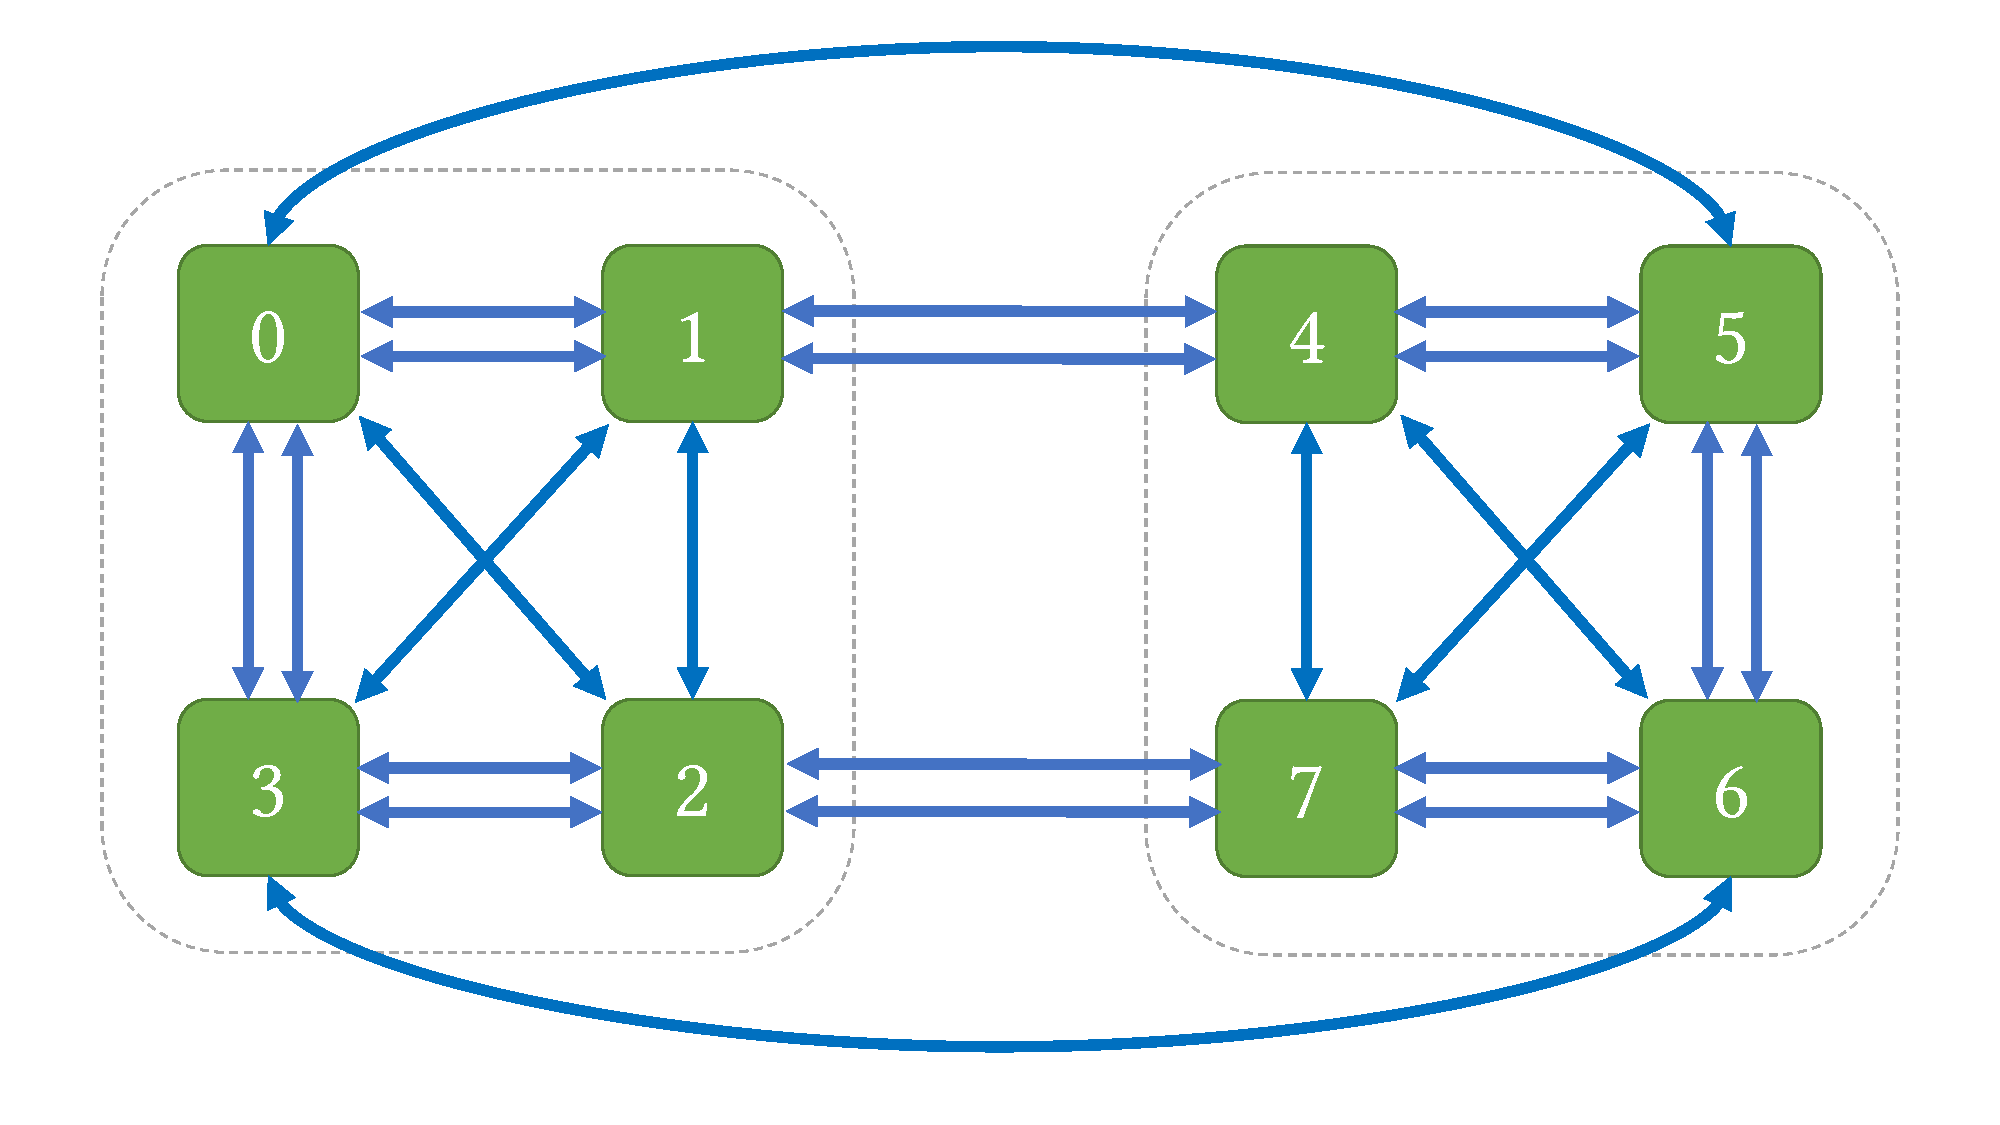
\includegraphics[page=1,width=\columnwidth]{figures/topos.pdf}
\caption{NVLink topology of an NVIDIA DGX-1.}
\label{fig:dgx1-topo}
\end{figure}
%\todo{the grey box indicating a socket has a low contrast when printed. colours for two different rings should have higher contrast (blue and orange perhaps?)}

% explain our approach
In this paper, we automatically synthesize high-performance communication kernels. 
Given a topology, specified as a graph with bandwidth constraints on nodes and edges, and a communication primitive, specified as the pre- and post-condition on data location and computation on it, we generate~(Section~\ref{sec:synthesis}) a quantifier-free SMT formula that captures the set of all feasible algorithms that implement the primitive on the input topology.
Exploring this space to appropriately minimize the number of communication steps or decrease the granularity of communication at each step, is a computationally difficult problem. We exploit
an SMT solver to synthesize algorithms that explore this tradeoff along the Pareto frontier between latency-optimality and bandwidth-optimality.
For every solution from the SMT solver, we automatically generate and lower~(Section~\ref{sec:lowering}) high-performance implementations.


% We approach this problem as a synthesis problem. Collective communication
% primitives can be specified in terms of pre- and post-conditions on which
% processes data resides on and optionally where a user specified reduction
% function has been applied. We encode pre- and post-conditions as well as actions
% to move data between processes as quantifier-free SMT formulas, which we solve
% using Z3. We further impose constraints on bandwidth usage based on the topology
% of the specific machine we are targeting and limit the number of steps for the
% whole algorithm. This gives us a way to explore the entire space of possible
% algorithms for implementing a given primitive on the target hardware.

% how do we make it scalable
When using SMT, finding the right encoding can make all the difference for the
feasibility of an approach. This paper details the important design choices in
our encoding that help it scale to all of our hardware targets. We use the SMT
encoding for \broadcasting collectives, such as \broadcast, while for \reducing
collectives, such as \reduce, we employ a reduction back to the synthesis
problem for \broadcasting collectives.
%A key observation is that topologies have natural symmetries. Our encoding exploits this symmetry to efficiently explore the space of algorithms without sacrificing satisfiability.
This reduction generalizes a well known fact that some \reducing collectives may
be produced by inverting a \broadcasting one, e.g. \reduce by inverting \broadcast.

%This allows us to reuse
%the synthesis of certain primitives such as \allreduce, further improving our
%scalability. 
%\todo{"time time-reversed mirror-image", huh? find easier to understand wording.}
%\todo{what do you mean by "modularize"? it's more like we reduce (no pun intended) the problem of reduction to broadcasting, which is the wording used later in bullet points}

% This informed an optimization in
% our encoding, that allows us to make reasoning about which GPUs data has been
% reduced implicit.

%\todo{This is quite vague right now.}

% The ability to control the number of steps an algorithm must execute in gives us
% a novel capability for trading off between latency and bandwidth optimality. By
% synthesizing a range of algorithms at different points in this space we can use
% the best algorithm for any given message size. While MPI implementations and
% NCCL both switch between algorithms based on message size, our synthesis
% approach allows us to do so in a much more fine grained manner. We show that
% this enables our algorithms to provide better performance than NCCL at all
% message sizes. \todo{Update this claim with truth.}

We implement our approach in a tool called \toollong{}~(\tool{}),
which probes the target hardware topology, synthesizes algorithms for
it using Z3~\cite{z3} and finally generates CUDA code that efficiently implements that algorithm.  These algorithms are
synchronous; at every step of the algorithm, one or more of the nodes
send and/or reduce data from others.
%\todo{"CUDA code"=>hardware dependent code? we have AMD GPUs. From saemal: AMD runs CUDA. OpenCL is another possibility but no one really uses it.}

% algorithmic novelty
Some of the algorithms we synthesize are novel, with no known counterparts in
the literature occupying the same latency-bandwidth tradeoff. For example, we
have produced a latency-optimal 2-step (4-step) algorithm for 
the \allgather (\allreduce) primitive in the DGX-1 topology (Figure~\ref{fig:dgx1-topo}) and
a bandwidth-optimal 3-step (6-step) algorithm for the \allgather (\allreduce) primitive on the 
same topology.  In addition to providing novel
algorithms, our approach informs us when a combination of bandwidth and number
of steps is \emph{not possible}. This makes our synthesis approach a tool for
probing the algorithmic properties that a given topology provides, which is
useful for co-design of hardware interconnects with communication libraries.
%\todo{"occupying the same latency-bandwidth tradeoff": exhibiting? and being different isn't necessarily good, we want more bandwidth with the same latency or lower latency with the same bandwidth.}
%\todo{tell reader that the "number of steps" correlate with latency?}
% results
Our evaluation~(Section~\ref{sec:evaluation}) shows us that this approach scales and beats NCCL in almost all cases. 


To summarize, the contributions of our paper are as follows:
\begin{itemize}
    \item A formalization of the synthesis problem for \broadcasting collectives.
    \item A general strategy for encoding the synthesis problem for
    collective communications algorithms into the quantifier-free linear integer
    arithmetic (QF\_LIA) sub-logic of the SMT-LIB logic.
    \item A reduction from the synthesis problem for \reducing collectives to that for \broadcasting collectives.
    % \item Explanations of some novel algorithms our synthesis has produced.
    \item A description of how \tool{} generates efficient code for the algorithms we synthesize on nodes with NVIDIA or AMD GPUs.
    \item An evaluation of \tool's generated algorithms on common server topologies for deep learning workloads and a comparison against NCCL.
\end{itemize}

%\todo{Paper structure paragraph?}

%%% Local Variables:
%%% mode: latex
%%% TeX-master: "paper"
%%% End:
